\documentclass{beamer}
\usepackage[utf8]{inputenc}

\usetheme{Madrid}
\usecolortheme{default}
\usepackage{amsmath,amssymb,amsfonts,amsthm}
\usepackage{txfonts}
\usepackage{tkz-euclide}
\usepackage{listings}
\usepackage{adjustbox}
\usepackage{array}
\usepackage{tabularx}
\usepackage{gvv}
\usepackage{lmodern}
\usepackage{circuitikz}
\usepackage{tikz}
\usepackage{graphicx}
\usepackage{amsmath}

\setbeamertemplate{page number in head/foot}[totalframenumber]

\usepackage{tcolorbox}
\tcbuselibrary{minted,breakable,xparse,skins}



\definecolor{bg}{gray}{0.95}
\DeclareTCBListing{mintedbox}{O{}m!O{}}{%
  breakable=true,
  listing engine=minted,
  listing only,
  minted language=#2,
  minted style=default,
  minted options={%
    linenos,
    gobble=0,
    breaklines=true,
    breakafter=,,
    fontsize=\small,
    numbersep=8pt,
    #1},
  boxsep=0pt,
  left skip=0pt,
  right skip=0pt,
  left=25pt,
  right=0pt,
  top=3pt,
  bottom=3pt,
  arc=5pt,
  leftrule=0pt,
  rightrule=0pt,
  bottomrule=2pt,
  toprule=2pt,
  colback=bg,
  colframe=orange!70,
  enhanced,
  overlay={%
    \begin{tcbclipinterior}
    \fill[orange!20!white] (frame.south west) rectangle ([xshift=20pt]frame.north west);
    \end{tcbclipinterior}},
  #3,
}
\lstset{
    language=C,
    basicstyle=\ttfamily\small,
    keywordstyle=\color{blue},
    stringstyle=\color{orange},
    commentstyle=\color{green!60!black},
    numbers=left,
    numberstyle=\tiny\color{gray},
    breaklines=true,
    showstringspaces=false,
}


\title 
{1.7.7}
\date{August 31,2025}


\author 
{Abhiram Reddy-AI25BTECH11021}



\begin{document}


\frame{\titlepage}
%------------------------------------
\begin{frame}{Problem Statement}
\textbf{Find the value of \( p \)} such that the points:
\[
A(2,1), \quad B(p, -1), \quad C(-1,3)
\]
are \textbf{collinear}, using \textcolor{blue}{matrices and echelon form}.
\end{frame}

%------------------------------------
\begin{frame} {Step 1: Vector Form}
Two vectors from point \( A \):

\[
\overrightarrow{AB} = (p - 2, -2), \qquad \overrightarrow{AC} = (-3, 2)
\]

Construct a matrix:
\[
M = 
\mat{
p - 2 & -2 \\
-3 & 2
}
\]

We will use row reduction (echelon form) to find when the rows are linearly dependent.
\end{frame}

%------------------------------------
\begin{frame}{Step 2: Row Reduction}
Let:
\[
R_1 = [p - 2 \quad -2], \quad R_2 = [-3 \quad 2]
\]

Apply:
\[
R_2 \rightarrow R_2 + \frac{3}{p - 2} R_1
\]

Compute:
\[
R_2 = [0 \quad 2 - \frac{6}{p - 2}]
\]

Set the second row to zero:
\[
2 - \frac{6}{p - 2} = 0
\]
\[
2(p - 2) = 6 \Rightarrow 2p - 4 = 6 \Rightarrow 2p = 10 \Rightarrow \boxed{p = 5}
\]
\end{frame}

%------------------------------------
\begin{frame}{Conclusion}
\begin{block}{Final Answer}
\[
\boxed{p = 5}
\]
\end{block}

For \( p = 5 \), the points \( A, B, C \) are collinear since the row-reduced matrix becomes dependent (second row becomes zero).
\end{frame}


\begin{frame}[fragile]
    \frametitle{C Code for echelon matrix }

    \begin{lstlisting}

#include <stdio.h>

void echelonForm(double matrix[2][2]) {
    // Assuming matrix is 2x2
    double factor;

    // Make the first element of second row zero by row operation
    if (matrix[0][0] == 0) {
        printf("Cannot perform elimination as pivot is zero.\n");
        return;
    }
    
    factor = matrix[1][0] / matrix[0][0];

    // Subtract factor * first row from second row
    matrix[1][0] = matrix[1][0] - factor * matrix[0][0];
    matrix[1][1] = matrix[1][1] - factor * matrix[0][1];
}
\end{lstlisting}
\end{frame}

\begin{frame}[fragile]
    \frametitle{C Code for echelon matrix }

    \begin{lstlisting}

int main() {
    double p;
    printf("Enter value for p: ");
    scanf("%lf", &p);

    // Create matrix with rows [p-2, -2] and [-3, 2]
    double matrix[2][2] = {
        {p - 2, -2},
        {-3, 2}
    };
    \end{lstlisting}
\end{frame}
\begin{frame}[fragile]
    \frametitle{C Code for echelon matrix }

    \begin{lstlisting}

    printf("Original matrix:\n");
    for(int i=0; i<2; i++) {
        for(int j=0; j<2; j++) {
            printf("%8.3f ", matrix[i][j]);
        }
        printf("\n");
    }

    echelonForm(matrix);

    printf("\nMatrix after echelon form operation:\n");
    for(int i=0; i<2; i++) {
        for(int j=0; j<2; j++) {
            printf("%8.3f ", matrix[i][j]);
        }
        printf("\n");
    }

    if (matrix[1][1] == 0) {
        printf("\nRows are linearly dependent; points are collinear for p = %.3f\n", p);
    } else {
        printf("\nRows are not linearly dependent; points are NOT collinear for p = %.3f\n", p);
    }

    return 0;
}

    \end{lstlisting}
\end{frame}

\begin{frame}[fragile]
    \frametitle{Python Code for plot}
    \begin{lstlisting}
import matplotlib.pyplot as plt

# Points
A = (2, 1)
B = (5, -1)
C = (-1, 3)

# Plot points
plt.scatter(*A, color='red', label='A(2,1)')
plt.scatter(*B, color='blue', label='B(5,-1)')
plt.scatter(*C, color='green', label='C(-1,3)')

# Plot line through A and C
x_values = [A[0], C[0]]
y_values = [A[1], C[1]]
plt.plot(x_values, y_values, 'k--', label='Line through A and C')

    \end{lstlisting}
\end{frame}

\begin{frame}[fragile]
    \frametitle{Python Code for plot}
    \begin{lstlisting}

plt.legend()
plt.grid(True)
plt.xlabel('x')
plt.ylabel('y')
plt.title('Collinear Points for p=5')

# Save the plot as an image file
plt.savefig('python_plot.png')  # Saves to current directory

plt.show()


    \end{lstlisting}
\end{frame}




\begin{frame}{Plot}
    \centering
    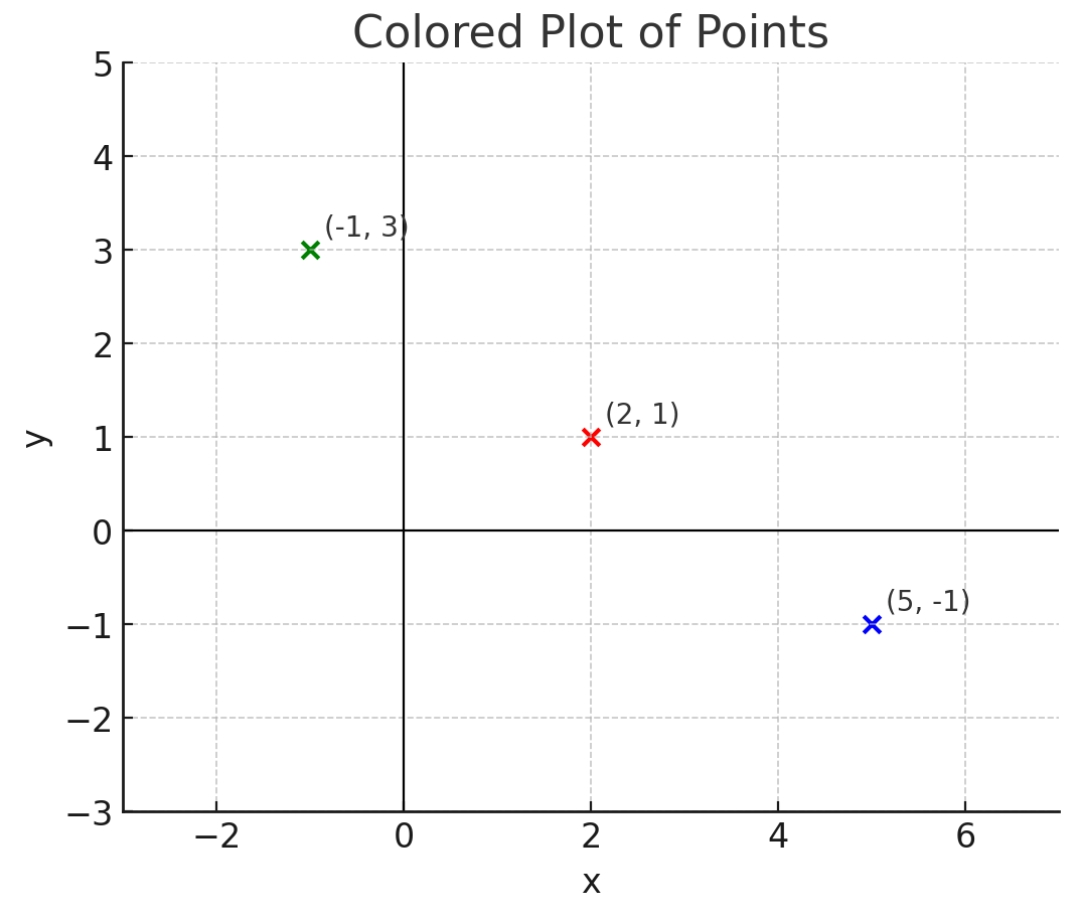
\includegraphics[width=\columnwidth, height=0.8\textheight, keepaspectratio]{figs/python_plot.png}     
\end{frame}


\end{document}